




\subsection{Hedge Fund 对冲基金}


\subsubsection{Characteristics of hedge funds}
\begin{table}[h]
    \centering
    \caption{Comparison between Hedge Funds and Mutual Funds}
    \begin{tabular}{@{}lcc@{}}
        \toprule
         & Hedge Funds & Mutual Funds \\
        \midrule
        Characteristic & Private vehicles & General Public \\
        Regulation & Less Regulated & Severe Regulation \\
        Leverage & High & Low \\
        Strategy & Both long and short positions & Long - bias \\
        Transparency & Low (keep from mimicking or front running) & High \\
        Fees Charge & 2 and 20, 1 and 10 & Only Management Fees \\
        Performance evaluation & Expect out - sized return & Well defined performance target \\
        \bottomrule
    \end{tabular}
\end{table}



\subsubsection{Databases of hedge funds}
\begin{itemize}
\item Self-Selection bias (selection bias): Manager who have funds with an unimpressive track record will not wish to have that information exposed. In other words, there may well be a tendency to "put the best face forward".
\item Backfill bias: When a new fund replaces a deleted fund in an index, the past performance of the new fund is inserted.
\item Issues from illiquid assets and the solutions
    \begin{itemize}
    \item Correlation with other asset classes will be lowered (appearance of low systematic risk)
        \begin{itemize}
        \item Using regression with additional lags of the market factors and summing the coefficient across lags.
        \end{itemize}
    \item Volatility will be lowered (low total risk)
        \begin{itemize}
        \item Taking autocorrelation into account when extrapolating risk to longer horizons.
        \end{itemize}
    \end{itemize}
\end{itemize}



\subsubsection{Evolution of hedge fund industry}
\begin{itemize}
\item Early days (1987-1994): show a very sizeable performance gap between the large hedge funds and the SNP.
\item Fall of LTCM (1998): a significant reduction in investors' appetite.
\item Burst of the dot-com bubble (2000-2001)
\item The arrival of institutional investors (2002-2010): Investors in hedge funds thus shifted from exclusively private wealth to institutions, including foundations, endowments, pension funds, and insurance companies.
    \begin{itemize}
    \item They entered hedge fund market in search of alternative sources of return away from the equity market.
    \end{itemize}
\end{itemize}



\subsubsection{Hedge fund strategies}
\begin{itemize}
\item Directional hedge fund styles:
    \begin{itemize}
    \item Managed futures
    \item Global Macro
    \end{itemize}
\item Event-driven styles:
    \begin{itemize}
    \item Merger arbitrage
    \item Distressed securities
    \end{itemize}
\item Relative value and arbitrage-like strategies:
    \begin{itemize}
    \item Fixed income arbitrage
    \item Convertible arbitrage
    \item Long/short equity
    \end{itemize}
\item Niche strategies:
    \begin{itemize}
    \item Dedicated short
    \item Emerging markets
    \item Equity market neutral strategy
    \end{itemize}
\item Directional hedge fund styles:
    \begin{itemize}
    \item Managed futures （CTAs, commodity trading advisors）: focus on investing in listed bond, equity, commodity futures, and currency markets, globally.
        \begin{itemize}
        \item Systematic trading programs are employed. Managed futures fund managers rely upon historical price data and market trends.
        \item A significant amount of leverage is often employed since the strategy involves the use of futures contracts.
        \end{itemize}
    \item  Global macro:
        \begin{itemize}
        \item Focuses on identifying extreme price valuations and leverage is often applied on the anticipated price movements in equity, currency, interest rate and commodity markets.
        \item employs a top-down global approach to concentrated on forecasting how political trends and global macroeconomic events affect the valuation of financial instruments.
        \item Profits can be made by correctly anticipating price movements in global markets and having the flexibility to use a broad investment mandate, with the ability to hold positions in practically any market with any instrument.
        \end{itemize}
    \item Similarity between global macro and managed futures: these managers behave like asset allocators taking bets in different markets utilizing a range of strategies opportunistically.
    \end{itemize}
\item Event-driven styles:
    \begin{itemize}
    \item Merger arbitrage: attempts to capture the spreads in merger or acquisition transactions involving public companies after the terms of the transaction have been announced.
    \item In a fixed exchange ratio stock merger, one would go long one and short another one according to the merger ratio, in order to isolate the spread and hedge out market risk.
    \item Distressed securities: This strategy invests across the capital structure of companies subject to financial or operational distress or bankruptcy proceedings. Such securities often trade at discount to intrinsic value due to difficulties in assessing their proper value, lack of research coverage, or an inability of traditional investors to continue holding them.
        \begin{itemize}
        \item Distressed managers ty pically attempt to profit on the issuer's ability to improve its operation or the success of the bankruptcy process that ultimately leads to an exit strategy.
        \item The main feature of this investment strategy is long exposure to credit risk of corporations with very low credit ratings.
        \end{itemize}
    \item This strategy is generally long-biased in nature.
    \item There is some evidence of nonlinearity between the two return series, particularly at the extreme tails (mostly as tail risk that shows up under extreme market conditions).
    \item Unlike trend followers, who tend to benefit from extreme moves, event-driven funds are hurt by extreme moves.
    \end{itemize}
\item Relative value and arbitrage-like strategies:
    \begin{itemize}
    \item Fixed income arbitrage: attempts to generate profits by exploiting inefficiencies and price anomalies between related fixed income securities.
    
    \begin{table}[h]
        \centering
        \caption{Financial Instrument Strategies}
        \begin{tabular}{@{}lp{7cm}@{}}
            \toprule
            Instrument & Strategy (Bet) \\
            \midrule
            Swap spread trade & Change in spread of fixed side and floating side \\
            Yield - curve spread trades & Deviate from overall yield curve only for short - run \\
            Mortgage spread trades & Prepayment rates \\
            Fixed income volatility trades (Gamma, Vega) & Implied volatility of interest \\
            Capital structure or credit arbitrage trades & Mispricing among different types of securities (equity and debt) \\
            \bottomrule
        \end{tabular}
    \end{table}
    \item Convertible arbitrage: aims to profit from the purchase of convertible securities and the subsequent shorting of the corresponding stock when there is a pricing error.
        \begin{itemize}
        \item The number of shares shorted is based on a delta neutral or market neutral ratio. As a result, under normal market conditions, the arbitrageur generally expects the combined position to be insensitive to fluctuations in the price of the underlying stock.
        \item Pricing anomaly
        \item Gamma/vega trading
        \end{itemize}
    \item Long/short equity: invests in both long and short sides of equity markets, generally focusing on diversifying or hedging across particular sectors, regions or market capitalizations.
        \begin{itemize}
        \item Managers typically have the flexibility to shift from value to growth; small to medium to large capitalization stocks; and net long to net short.
        \item 30-40\% of hedge funds are long/short.
        \end{itemize}
    \end{itemize}
\item Niche strategies:
    \begin{itemize}
    \item Dedicated short: takes more short positions than long positions and earn returns by maintaining net short exposure in long and short equities.
        \begin{itemize}
        \item The returns are negatively correlated to equities.
        \end{itemize}
    \item Emerging markets: invests in currencies, debt, equities, and other instruments of countries with emerging or developing markets.
        \begin{itemize}
        \item The markets are typically measured by GDP per capita. Such countries are considered to be in a transitional phase between developing and developed status.
        \end{itemize}
    \item Equity market neutral strategy: there is no single common risk factor that drives the return behavior of equity market neutral funds. Return behavior suggests that different funds apply different trading strategies with a similar goal of achieving almost zero beta(s) against a broad set of equity indices.
    \end{itemize}
\item Exercise
    \begin{itemize}
    \item Samantha Moore manages a hedge fund for a mid-sized money management firm. The fund frequently changes styles according to identified profit opportunities. At the beginning of the year, the fund took a long position in 10-year subordinated 8\% coupon debt issued by a firm expected to undergo reorganization under Chapter 11. Moore felt that analysts had been paying too little attention to the issuer.
    
    Six months later, the fund completed a second transaction involving a long position in Swiss Francs and a short position in Japanese Yen based on forecasted movements in interest rates in the two countries. What two hedge fund strategies are most likely being employed by Moore's hedge fund?

A. Distressed securities strategy and equity long/short strategy.

B. Fixed-income arbitrage and global macro strategy.

C. Distressed securities strategy and global macro strategy.

D. Fixed-income arbitrage and equity long/short strategy.

\item Answer: C

解析:基金购入了一只次级债，公司正在进行破产充足，此为破产公司证券策略:六个月后，基金进入了瑞士法郎的多头和日元的空头，主要是在宏观上对这两个国家的货币做出相对的选择，此为全球宏观策略。


    \end{itemize}
\end{itemize}



\subsubsection{Hedge fund performance}
\begin{itemize}
\item In practice, evaluating hedge funds poses considerable practical challenges:
    \begin{itemize}
    \item The risk profile of hedge funds may change rapidly.
        \begin{itemize}
        \item Take time-varying bets on different risk factors and the risk profile is nonlinear and responsive to changing equity market conditions.
        \item Considerable ability to manipulate conventional performance measures.
        \item Expose the fund to infrequent but severe losses.
        \end{itemize}
    \item Hedge funds tend to invest in illiquid assets.
    \item When hedge funds are evaluated as a group, survivorship bias can be a major consideration, because turnover in this industry is higher than for investment companies such as mutual funds.
    \end{itemize}
    

\end{itemize}



\subsubsection{Convergence of risk factors}
\begin{itemize}
\item An important feature that attracts investors to the hedge fund industry is the variety of strategies hedge fund managers deploy and the diversity of assets to which these strategies are applied.
\item However, during times of stress, portfolio diversification implodes, and seemingly diverse hedge fund portfolios converge in terms of risk factors.
\item March to April period in 1994, unexpected hike in interest rate policy by the US Federal Reserve.
\item August 1998 leading up to the collapse of LTCM.
\item 2007-2008 financial crisis: "forced liquidation" of leveraged positions driven by a combination of rising margin requirements, borrowing costs and investors withdrawing their equity.
\item The risk behind cannot be easily mitigated by simply spreading one's capital to different hedge fund strategies.
\item The need to consider hedging a tail risk event in a hedge fund portfolio is clear.
\item The risk management of hedge fund portfolios must take into consideration nonlinear risks such as rare but dramatic market events the manifestation of which can take place on either the asset side and/or the liability side of a hedge fund's balance sheet.
\end{itemize}



\subsubsection{Agency problem}
\begin{itemize}
\item There is a concern about the asymmetry in risk sharing between principal and agent inherent in variable compensation schemes of which hedge fund style incentive fees is one such variation.
\item The problem arises when the incentive fee which hedge fund managers are entitled to, typically at 15-20\% of new profits, ends up enticing a fund manager to take unreasonable bets.
    \begin{itemize}
    \item If fund has a negative return, managers still obtain management fee.
    \end{itemize}
\item How to reduce asymmetric risk:
    \begin{itemize}
    \item High water mark.
    \item Lower incentive fees for fund managers.
    \item High fund closure costs.
    \item Force a fund manager to invest in any fund that he manages.
    \end{itemize}
\end{itemize}



\subsection{Performing Due Diligence on Specific Managers and Funds}



\subsubsection{Due diligence basics}
\begin{itemize}
\item Due diligence is the term used to describe the process of evaluation and analysis that an investor follows to get comfortable with a strategy, manager, and a fund prior to making an investment.
\end{itemize}



\subsubsection{Reasons for failures of funds in the past}
\begin{itemize}
\item Bad investment decisions: funds can make several compounded bad decisions or just a few concentrated calls on the markets or individual securities that perform very poorly.
\item Fraud: accounting frauds, valuation frauds, or misappropriation of funds.
\item Extreme events: excessive leverage, improbable probabilities, unexpected events and tail risk.
\item Lack of liquidity:
    \begin{itemize}
    \item A flood of unanticipated withdrawals of capital at the least opportune time.
    \item Squeeze.
    \item When liquidity dries up, funds cannot meet redemptions.
    \end{itemize}
\item Poor controls: a lack of supervision or compliance controls related to insider trading.
\end{itemize}




\subsubsection{Elements of the due diligence process}
\begin{itemize}
\item Today, both managers and investors spend a great deal of time trying to learn where a manger's "edge" is coming from and that their investment is safeguarded and properly valued.
\item The goal is to find out what is really going on at the fund and not just have a pitch book recitation by the investor relations staff.
\begin{center}
    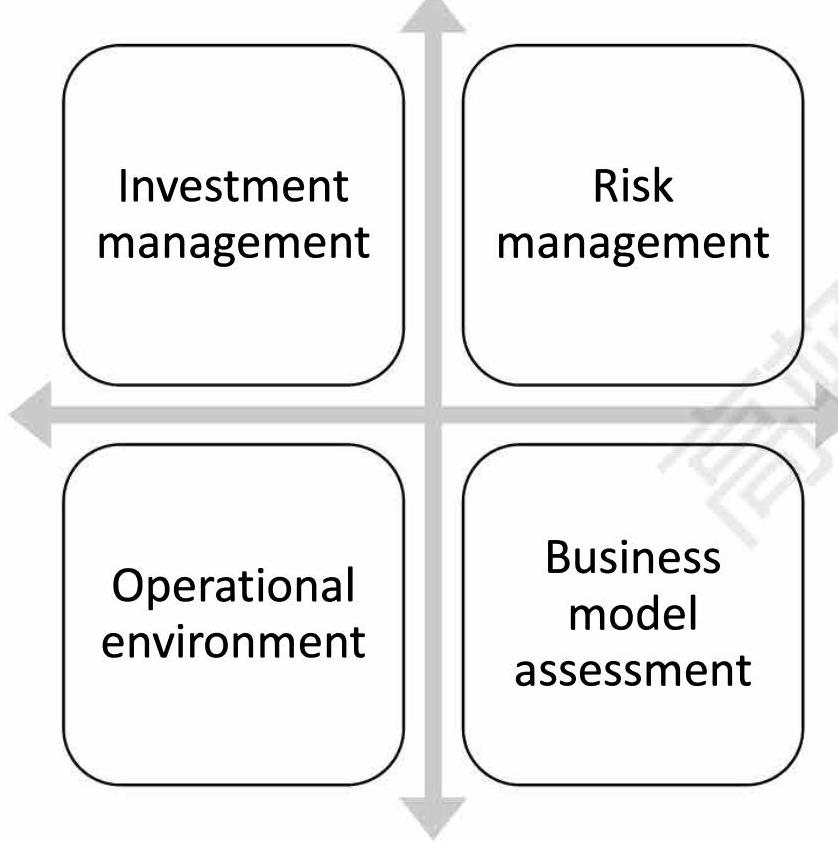
\includegraphics[width=0.4\textwidth]{images/Elements.jpg}
    \end{center}    
    

\end{itemize}



\subsubsection{Investment management}
\begin{itemize}
\item Strategy:
    \begin{itemize}
    \item Manager's self-described style
    \item Concentrated positions
    \item Turnover and number of days to liquidate
    \item Stop losses
    \item Short sales used
    \item OTC derivatives
    \item Central trading desk
    \item Generate returns for existing investors or grow AUM?
    \end{itemize}
    
\item Equity ownership: some firms do not share equity ownership among the portfolio managers or traders in the firm; other firms use equity ownership as a key feature of their professional talent retention program and to attract and groom new talent for future leadership position.


\item Track record reliable
    \begin{itemize}
    \item Whether the track record is comparable to similar strategies
    \end{itemize}
    
\item Managers:
    \begin{itemize}
    \item Newer managers: ask former colleagues, partners, managers, clients, or other independent parties.
    \item Established managers: motivation, behavior during crisis or stress periods; ability to communicate to investor.
    \end{itemize}
    

\end{itemize}



\subsubsection{Risk management evaluation}
\begin{itemize}
\item Risk (Assessment, measurement, monitoring, mitigating)
\item Potential risks that a strategy will be exposed and additional idiosyncratic risks
\item Inputs and assumptions used in the firm's risk models
\item Written policies and procedures to monitor and measure each of the applicable risk
\item Security valuation
\item Portfolio leverage and liquidity
\item Tail risk exposure (Return distribution, skewness or kurtosis.)
\item Risk reports (Review and revise on a regular basis)
\item Consistency of the fund terms with the investment strategy.
\end{itemize}



\subsubsection{Operational environment}
\begin{itemize}
\item Internal control assessment
    \begin{itemize}
    \item Qualifications of people at the fund
    \item The quality of the written policies and procedures
    \item The ability of the team to execute, fund's exposure to derivative counterparties
    \item The protections provided by its governance structure
    \item In-house compliance or outsourced relationship with a compliance service provider
    \end{itemize}
\item Documents and disclosure
    \begin{itemize}
    \item An investor needs to verify with the listed law firm in the fund documents that they were responsible for the original content and for any updates.
    \item Fund offering memo, subscription agreement, limited partnership agreement, investment management agreement, Form ADV and website are all saying the same thing at the same point in time.
    \item Either insufficient or extremely broad risk disclosure
    \item Check the equity section to see if the general partner is continuing to invest in the fund
    \end{itemize}
\item Service provider evaluation

\end{itemize}



\subsubsection{Business model risk and fraud risk}
\begin{itemize}
\item Business model risk: deals with the risks encompassed in simply running the business of being a hedge fund.
    \begin{itemize}
    \item Adequate cash on hand.
    \item Where does the working capital come from.
    \item Succession plan (key person insurance).
    \item What happens if too many investors redeem at the same time.
    \item Break-even AUM.
    \end{itemize}
\item Fraud risk
\item Potential indicators:
    \begin{itemize}
    \item Lack of trading independence.
    \item Investor complaints about lack of liquidity.
    \item Litigation in civil court alleging fraudulent acts.
    \item Personal trading by managers
    \item Aggressive shorting and organized efforts to spread rumors.
    \item A high percentage of illiquid investment
    \end{itemize}
\end{itemize}



\subsubsection{Due diligence questionnaire}
\begin{itemize}
\item 1. Manager information
    \begin{itemize}
    \item a. Registration
    \item b. Ownership
    \item c. Organization
    \item d. References/ Background checks
    \item e. Track record
    \item f. Risk management
    \item g. Operations
    \item h. Service providers
    \item i. Contact details
    \end{itemize}
\item 2. Execution and trading
\item 3. Third-party research policy
\item 4. Compliance
\item 5. In-house legal
\item 6. Anti-money-laundering policy and procedures
\item 7. Disaster recovery and business continuity
\item 8. Insurance coverage and key man provisions
\item 9. Fund information
    \begin{itemize}
    \item a. Management and incentive fees
    \item b. Lock-up
    \item c. Subscriptions and redemptions
    \item d. Notice periods
    \item e. Fund directors or advisors
    \item g. Auditor
    \item h. Legal advisor
    \item k. Performance
    \item l. Capacity
    \item m. Gates and lock-ups
    \item n. Historical drawdown
    \item o. Use of managed accounts
    \item p. Investor mix
    \end{itemize}
\item 10. Investment process and portfolio construction
\item 11. Risk controls
    \begin{itemize}
    \item a. Concentration and diversification
    \item b. Liquidity
    \item c. Leverage
    \item d. Exposure to market risk factors
    \item e. Reporting
    \item f. Portfolio Greeks (duration, delta, beta, etc.)
    \end{itemize}
\item 12. Financial statements
    \begin{itemize}
    \item a. Year-end opinion
    \item b. Level 1, 2, 3 assets
    \item c. Interim statements
    \item d. Administrator reports
    \end{itemize}
    
\item 13. Terms and use of third-party marketers
\end{itemize}




\subsection{Finding Bernie Madoff: Detecting Fraud by Investment Managers}



\subsubsection{Fraud by investment managers}
\begin{itemize}
\item Ponzi scheme: on December 11, 2008, the securities and exchange commission (SEC) charged Bernard Madoff with securities fraud for committing an \$18 billion Ponzi scheme.
    \begin{itemize}
    \item The opportunities advisers have to exploit investors.
    \item The importance of limiting advisers' opportunistic behavior through either market or regulatory forces.
    \item In the U.S., the regulatory system protects investors primarily through mandatory disclosure.
    \end{itemize}
    
\item Fraud: fraud cases harm the firm's investment clients.
    \begin{itemize}
    \item Not include insider trading, short sale violations, brokerage fraud, or other crimes, unless they cause direct losses to the firm's investment clients.
    \end{itemize}
    
\end{itemize}



\subsubsection{Information disclosure}
\begin{itemize}
\item Form ADV:
    \begin{itemize}
    \item Investment advisers: any entity that receives compensation for managing securities portfolios or providing advice regarding individual securities.
        \begin{itemize}
        \item Firms: all mutual funds, nearly all institutional investment funds, and many hedge funds in the U.S.
        \end{itemize}
    \item Registered investment advisers: must file Form ADV to disclose past regulatory violations and potential conflicts of interest.
    


    \begin{table}[h]
        \centering
        \caption{Disclosure Items}
        \begin{tabular}{@{}p{3cm}p{2.5cm}p{2cm}p{2cm}p{2cm}p{2cm}@{}}
            \toprule
            Items 1 - 6 & Items 7 - 8 & Item 9 & Item 10 & Item 11 & Item 12 \\
            \midrule
            Descriptive information about a firm and its operations & Disclosure of certain conflicts of interest & Disclosure regarding the custody of clients’ assets & Disclosure of control person & Disclosure of past legal and regulatory violations & Small business \\
            \midrule
            \multicolumn{6}{l}{Schedules A - C: direct and indirect owners of a firm} \\
            \multicolumn{6}{l}{Schedule D: disclosure of affiliations with other financial firms} \\
            \bottomrule
        \end{tabular}
    \end{table}



    \end{itemize}
\item An investor who avoided the 5\% of firms with the highest ex ante predicted fraud risk would avoid 29\% of fraud cases and over 40\% of the dollar losses from fraud.
    \begin{itemize}
    \item Although to obtain these benefits, the investor would have to forgo investing with 5\% of non-fraudulent advisers.
    \end{itemize}
\end{itemize}


%✗
\subsubsection{Predicting fraud}

\begin{table}[ht]
    \centering
    \begin{tabular}{|l|l|c|}
    \hline
    \multirow{4}{*}{\textbf{Disciplinary history and regulatory and legal offenses}} 
        & Past fraud & $\times$ \\
        & Past affiliated fraud & $\times$ \\
        & Past regulatory & \checkmark \\
        & Past civil or criminal & \checkmark \\
    \hline
    \multirow{3}{*}{\textbf{Conflicts of interest}} 
        & Referral fees & \checkmark \\
        & Interest in transaction & \checkmark \\
        & Soft dollars & $\times$ \\
    \hline
    \multirow{4}{*}{\textbf{Monitoring}} 
        & Broker in firm & \checkmark \\
        & Investment Company Act & \checkmark \\
        & Custody & $\times$ \\
        & Dedicated CCO & $\times$ \\
    \hline
    \textbf{Client Type} & Hedge fund clients & $\times$ \\
    \hline
    \end{tabular}
    \caption{Compliance and Monitoring Overview}
    \end{table}


\begin{itemize}
\item 
\end{itemize}



\subsubsection{Compensated for fraud risk}
\begin{itemize}
\item Are investors compensated for fraud risk?
    \begin{itemize}
    \item High fraud risk may provide off-setting benefits that improve investment performance.
    \end{itemize}
\item Results: do not provide evidence that investors receive compensation for fraud risk.

\end{itemize}



\subsubsection{Barriers and costs}
\begin{itemize}
\item The lack of compensation for fraud risk does not necessarily imply that investors are irrational.
    \begin{itemize}
    \item Investors could be compensated in some other unmeasured fashion.
    \item Investors may predict fraud risk based on reputations, personal contacts, or other information
    \item Barriers to accessing Form ADV outweigh the benefits.
    \end{itemize}
\item For most investors, the cost of individually downloading thousands of Form ADV filings may well have exceeded the perceived benefits.
    \begin{itemize}
    \item To implement a fraud prediction model, an investor would have had to collect manually a large number of Form ADV filings, convert the filings into a database, and estimate a prediction model.
    \end{itemize}
\end{itemize}



\subsubsection{Improving ways}
\begin{itemize}
\item Allowing public access to historical Form ADV filings would reduce the marginal cost of increased enforcement by facilitating investors' use of these data.
\item This should reduce the marginal benefit to an investment adviser of committing fraud due to an increase in the probability of detection.
\item Improved public access to these disclosure data could reduce the occurrence of fraud.
\end{itemize}

